\documentclass[letterpaper, 10 pt, conference]{ieeeconf}
  % use above line letter sized paper
%\documentclass[a4paper, 10pt, conference]{ieeeconf}
  % Use this line for a4 paper
%\IEEEoverridecommandlockouts
  % Needed if you want to use the \thanks command
\overrideIEEEmargins
  % Needed to meet printer requirements.
\usepackage[utf8]{inputenc}
\usepackage{fullpage}
\usepackage{graphicx}
\usepackage{amsfonts}
\usepackage{amssymb}
\usepackage{amsmath}
\usepackage{latexsym}
\usepackage{enumerate}
\usepackage{float}
\usepackage[urlcolor=blue,colorlinks=true]{hyperref}
\usepackage{multirow}
\usepackage{leftidx}
\usepackage[backend=bibtex,
style=numeric
%style=alphabetic
%style=reading
]{biblatex}
\addbibresource{Sources.bib}

\title{Conversion of RGBD Images to Textured Triangle Meshes with GPU}
\author{Dalton Banks, Collin Boots}
\date{Nov 18, 2013}
\begin{document}
   \maketitle

As robots continue to be incorporated into human environments, the need for intelligent and high-speed reasoning about the objects around them increases dramatically. At the simplest level, mobile robots need to create a map of their environment for navigation. At a higher level, some robots need to recognize distinct objects in their environment, track object movement, and have some intuitive sense of object geometry that is easily stored and processed. Even more important is being able to efficiently generate this environment from sensor data in real time. Like the human brain, the robot should also be able to perform these low level functions with only minimal intervention from higher cognitive functions.\\

Previous work has demonstrated the diverse capabilities of depth cameras from generating highly accurate 3D surface models \cite{KinectFusion} to reliable 3D pose estimation \cite{Endres,Taguchi}. However, these efforts have collectively suffured from several limitations. Many algorithms attempt to store the generated environment as a RGB 3D point cloud (either pruned or complete), which is not easily adaptable to dynamic environments, requires exorbitant quantities of memory to store large environments, and provides no intuition to higher perception processes about distinct objects beyond a volumetric approximation. Other approaches have been able to store and merge the surface data more efficiently, but still regard the environement as a unified whole rather than discrete objects. These approaches may be sufficient for mapping static envirnoments, but provide only limited utility to more interactive robots and can actually hinder robots that reconfigure their surroundings (and hence invalidate part of their map).


\section*{Proposed Method}
A new method for storing and manipulating environement maps is proposed using triangle meshes to store all geometries. By extracting meaningful geometry from the RGB-D in the form of triangle meshes, a large number of advantages can be realized.
\begin{enumerate}
\item The storage format of a trinagle mesh is very efficient, allowing for large and detailed maps to be stored in memory constrained systems like small mobile robots. 
\item Mesh models provide a natural way of isolating distinct objects in the environment in a way that point clouds and surface maps cannot. 
\item Meshes are easy to manipulate, modify, and manifest in real time using well established computer graphics technology and open the problem to the wealth of domain knowledge from the gaming graphics industry. By representing the robot's environment in a similar manner to a game world, future robots may be able to more easily leverage the gaming industry's experience in intelligent actor design. 
\item By manipulating and moving meshes instead of erasing and redrawing portions of a discrete map or point cloud, map artifacts from more dynamic environements could be handled more gracefully and naturally.
\item Storing objects as distinct, flexible models provides a natural means of handling moving objects in lower level software, freeing higher level processes for reasonsing about object movement more abstractly.
\item Meshes provide an efficient and easy to process intuition of geometry to higher cognitive functions that may simply object recognition and manipulation tasks.
\item Meshes are very flexible in their ability to record complex geometries. By using a single storage format for all object types, many implementation efficiencies may be realized. Also, meshes provide a very straightforward tradeoff between simplicity and accuracy that can be situationally controlled.
\end{enumerate}
Using an off the shelf RGB-D depth camera like the Kinect to accomplish all of these goals also brings with it all the benefits explored in previous work: hardware simplicity, minimal integration complexity, and low cost. This work will focus primarily on generation of high-accuracy triangle meshes for a variety of scene complexities and difficult edge cases such as touching objects. Time and technology permitting, some of the potential advantages of the approach listed above will be explored and demonstrated.

\begin{figure}[!ht]
    \centering
    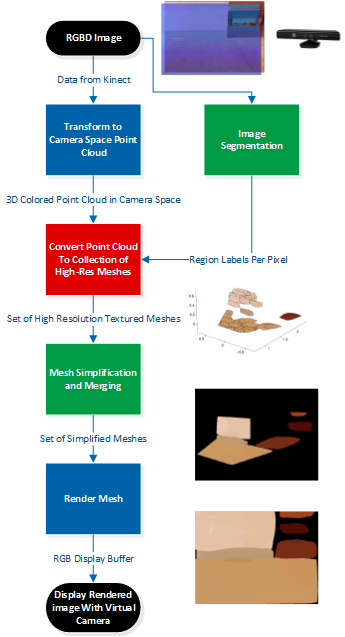
\includegraphics[scale=1.0]{pipelineflowchart.png}
    \caption{Pipeline Overview}
    \label{fig:pipeline}
\end{figure}

\printbibliography
\end{document}